\documentclass{article}

\usepackage{Engineering}
\pdftitle{Materials Lab}

% === TEXT ===
\title{\textbf{Materials Lab \\ HSLU, Semester 3}}
\author{Matteo Frongillo}
  \date{}

\begin{document}

\maketitle
\tableofcontents
\hfill
\section*{Exam}
10 pages individual summary, printed/written on paper (pictures allowed). Calculator, ruler, electrochemical series.
\pagebreak

\part{Physical metallurgy}
\section{Material classes, structural models, basic concepts}
\subsection{Material classes and typical properties}
\begin{center}
  \renewcommand{\arraystretch}{1.3}
  \begin{tabular}{|>{\bfseries}c|p{5.5cm}|}
    \hline
    Class & \textbf{4 Typical Properties} \\
    \hline
    Metals / Alloys & 
    1) Conductivity (electric, thermal) \newline
    2) Ductility / malleability \newline
    3) Castable \newline
    4) Shiny (reflective) \\
    \hline
    Ceramics & 
    1) High temperature resistance \newline
    2) Compression resistance \newline
    3) Insulator (electric, thermal) \newline
    4) Wear resistance \\
    \hline
    Polymers & 
    1) Cheap \newline
    2) Insulating (electric, thermal) \newline
    3) Longevity (corrosion resistance) \newline
    4) Moldable \\
    \hline
  \end{tabular}
\end{center}

\subsection{Structural model of metals}
In general, metals have:
\begin{itemize}
  \item \textbf{Metallic bonding}
  \item Good electrical and thermal conductivity
  \item Simple, densely packed crystal structures (atomic distances $\sim 0.1-0.2$ nm)
\end{itemize}

\begin{center}
  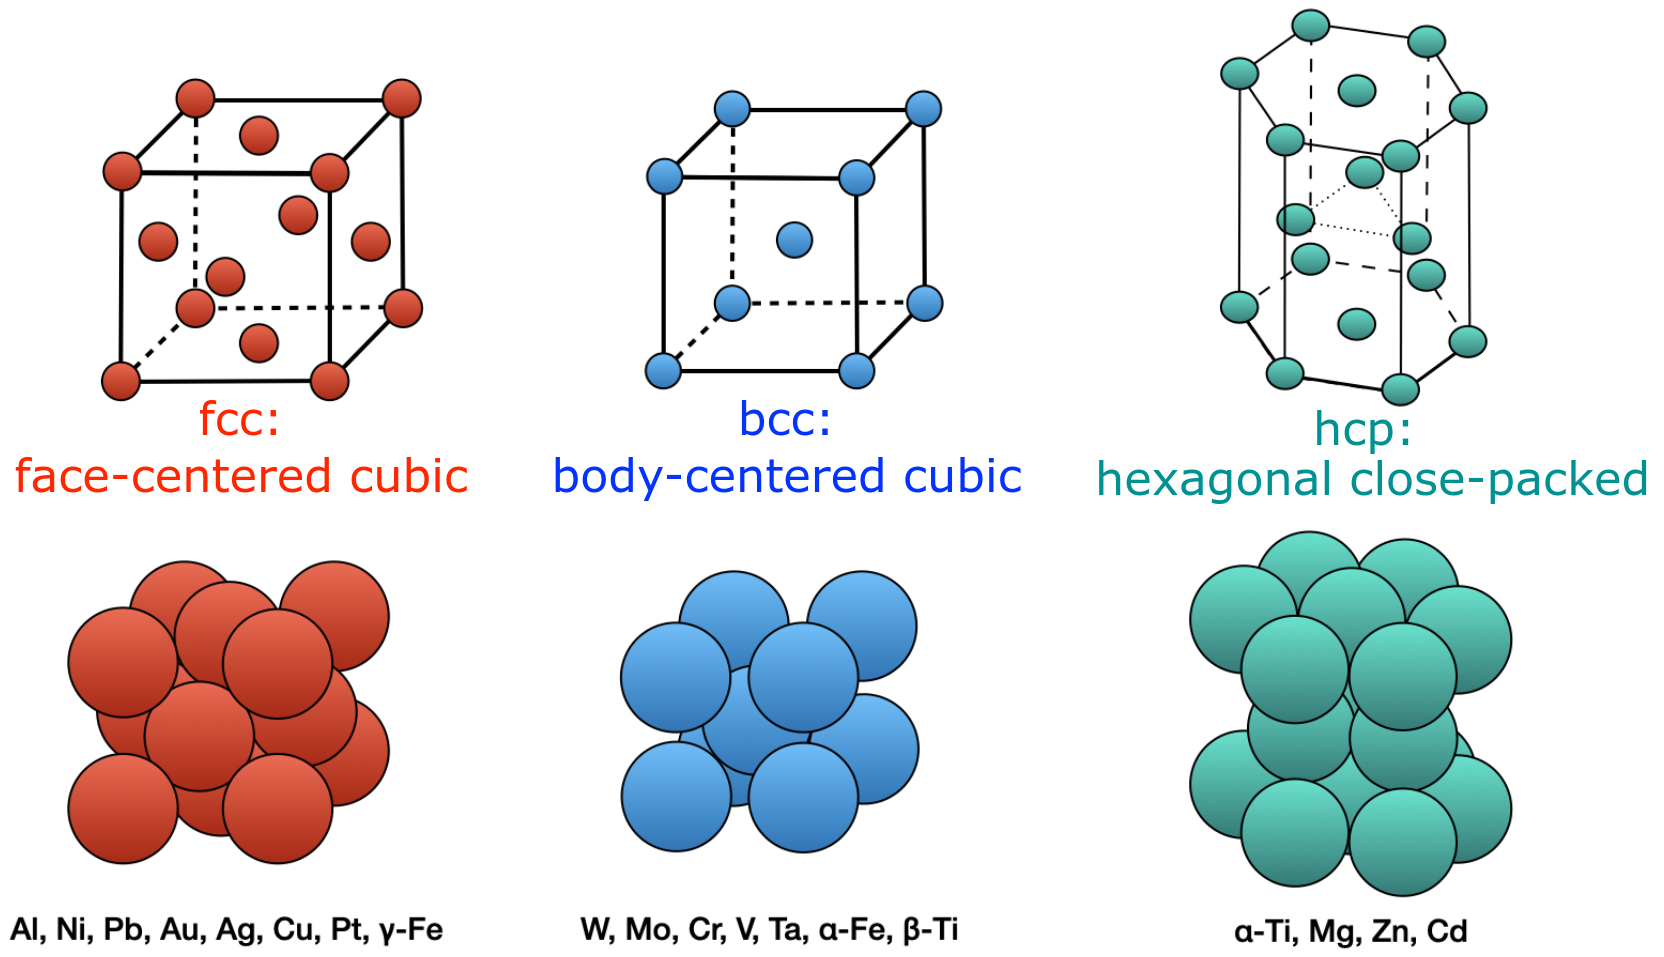
\includegraphics[width=0.8\textwidth]{media/fccbcchcp.png}
\end{center}

\begin{minipage}[t]{0.33\textwidth}
  \pph{FCC (Face-centered cubic)}
  \begin{itemize}
    \item Packing efficiency: 74\%
    \item Has many slip systems (12)
    \item Closest packed direction
  \end{itemize}
\end{minipage}%
\begin{minipage}[t]{0.33\textwidth}
  \pph{BCC (Body-centered cubic)}
  \begin{itemize}
    \item Packing efficiency: 68\%
    \item Has many slip systems (6)
    \item Not closest packed direction
    \item Cottrell atmosphere
  \end{itemize}
\end{minipage}%
\begin{minipage}[t]{0.33\textwidth}
  \pph{HCP (Hexagonal close-packed)}
  \vspace*{-0.45cm}
  \begin{itemize}
    \item Packing efficiency: 74\%
    \item Very few slip systems (3)
    \item Closest packed direction
  \end{itemize}
\end{minipage}

\figbox{$\text{Packing efficiency} = \dfrac{\text{Volume occupied by atoms in unit cell}}{\text{Total volume of unit cell}} \cdot 100\%$}
\newpage

\subsection{Structural model of ceramics}
In general, ceramics have:
\begin{itemize}
  \item \textbf{Ionic bonding, complex crystal structures (ceramics), amorphous (glasses)}
  \item Undoped: insulators (doped: semiconductors, superconductors or ionic conductors)
  \item Brittle, but high chemical and thermal resistance
  \item Wear-resistant, other special properties (e.g. ferro-/piezoelectricity)
\end{itemize}

\begin{figure*}[ht!]
  \centering
  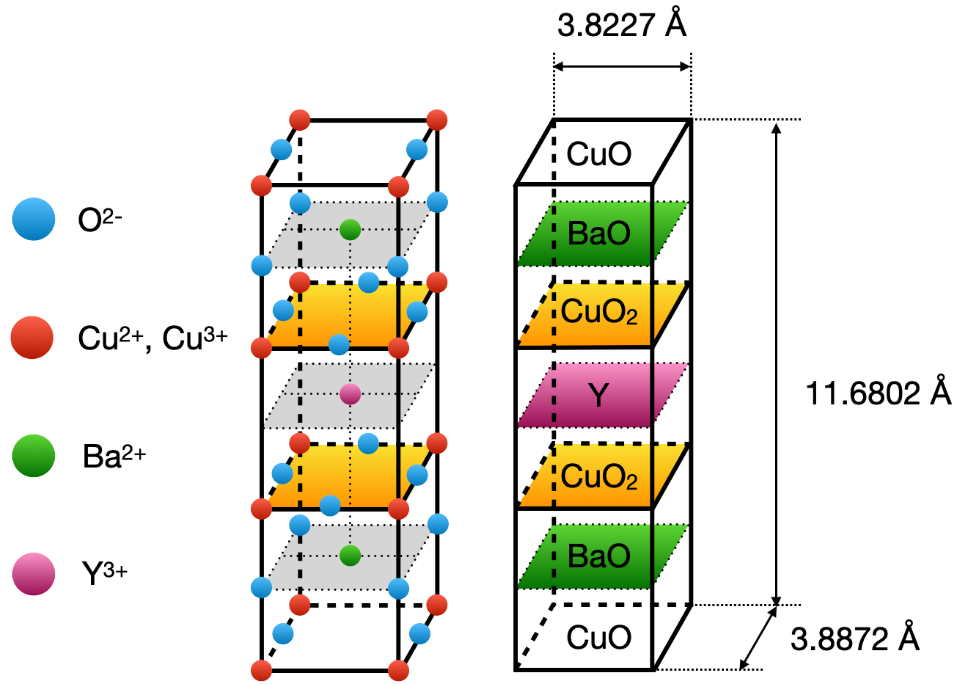
\includegraphics[width=0.6\textwidth]{media/ceramic_structure.png}
  \caption*{YBCO superconducting ceramic with layered perovskite-like structure}
\end{figure*}

\subsection{Structural model of polymers}
In general, polymers have:
\begin{itemize}
  \item Macromolecules ($10^3$ to $10^5$ C atoms)
  \item \textbf{Weaker intermolecular bonds} (strong atomic bond in molecular chain)
  \item Electrically and thermally insulating (without special modifications)
  \item Cheap, moldable, massive waste problem (e.g. ocean pollution)
  \item Matrix for many composite materials (recycling problem)
\end{itemize}
\begin{figure*}[ht!]
  \centering
  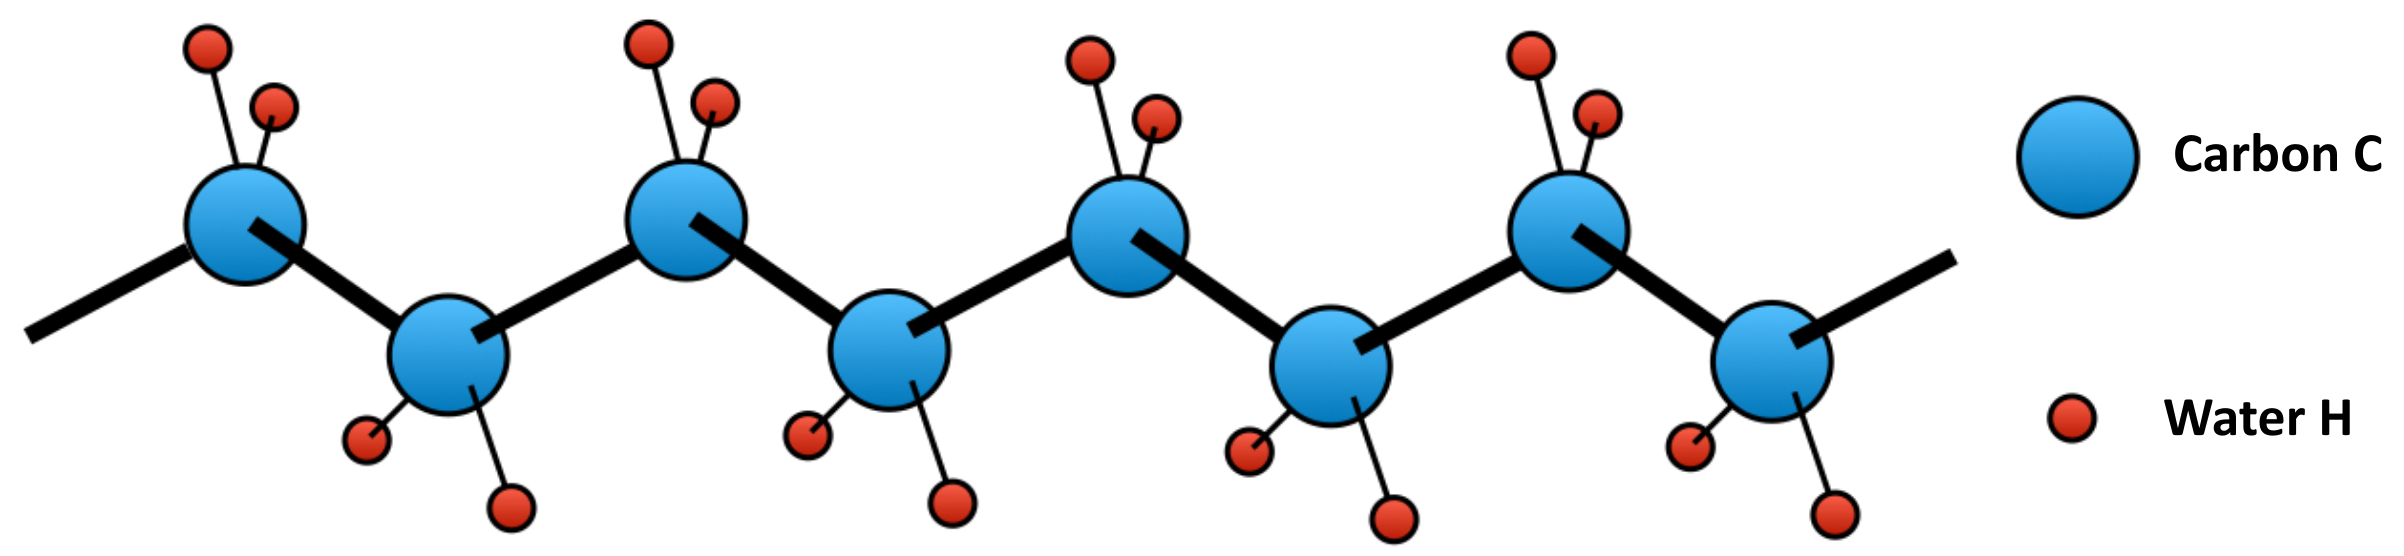
\includegraphics[width=0.8\textwidth]{media/polymer_structure.png}
  \caption*{Polymeric hydrocarbon chain}
\end{figure*}

\subsection{Amorphous and crystalline materials}
\begin{minipage}[t]{0.48\textwidth}
  \textbf{Amorphous materials}
  \begin{itemize}
    \item No crystal lattice (e.g. quartz glass, polymers)
    \item Atomic distances defined by chemical bonds
    \item Bond angles are variable
  \end{itemize}
\end{minipage}
\hfill
\begin{minipage}[t]{0.48\textwidth}
  \textbf{Crystalline materials}
  \begin{itemize}
    \item Crystal lattice (e.g. metals, ceramics, quartz)
    \item Atomic distances and bonding angles are defined
  \end{itemize}
\end{minipage}

\newpage
\begin{figure*}[ht!]
  \centering
  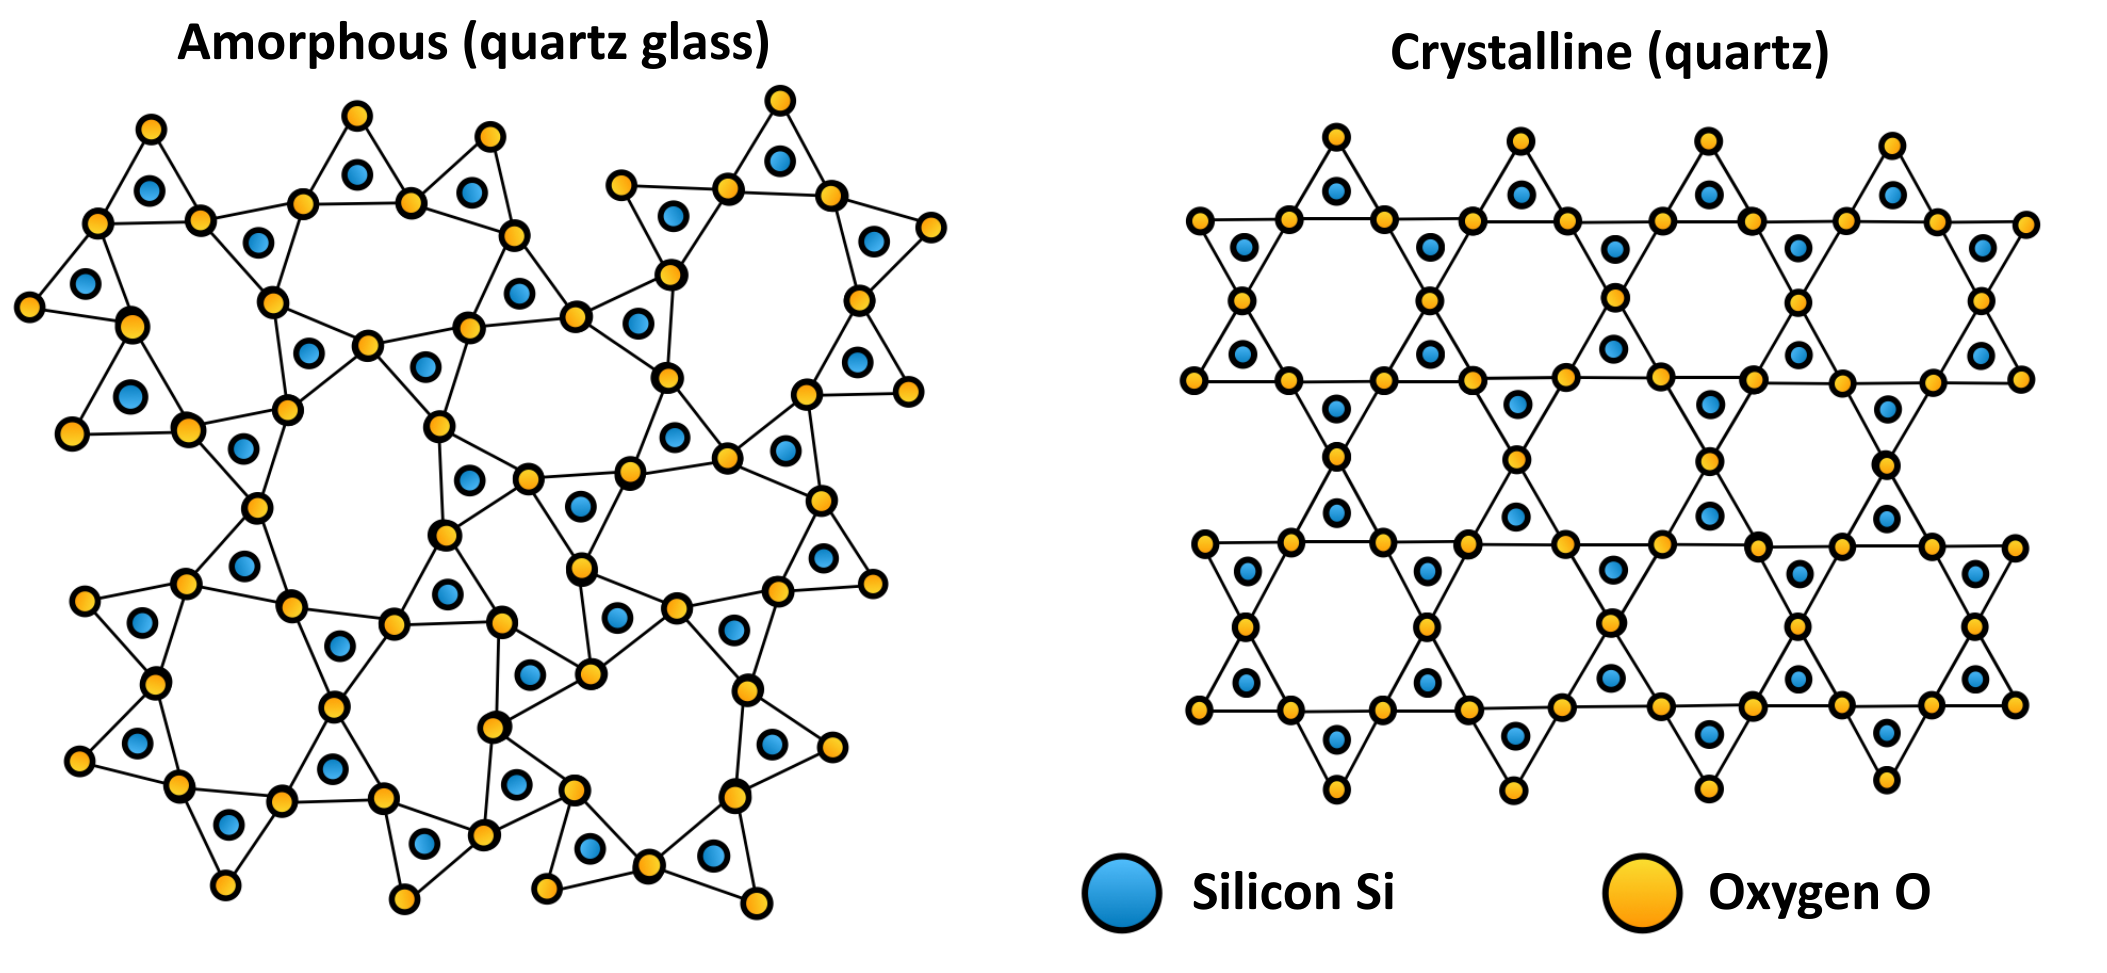
\includegraphics[width=0.8\textwidth]{media/amorph_cry.png}
\end{figure*}

\subsubsection{Polycrystalline materials}
Most metal components are polycrystalline (made of many grains/crystals),
i.e. they consist of countless microscopic crystals (crystallites, ``grains'').

\subsubsection{Monocrystalline materials}
\textbf{Only for special applications, expensive}
\begin{itemize}
  \item Single-crystal turbine blades ($T>1000^\circ C$, creep-resistant)
  \item Semiconductors, MEMS components made of silicon (e.g. gyroscopes in smartphones, accelerometers)
  \item Optical elements (e.g. laser crystals, $\lambda/4$ plates, crystals for frequency doubling of lasers)
\end{itemize}


\subsubsection{Amorphous materials}
\begin{itemize}
  \item Inorganic glasses (also Gorilla glass of smartphones)
  \item Metallic glasses (ferrous transformer sheet metal)
  \item Amorphous plastics (e.g. PMMA - plexiglass, COC, \dots)
\end{itemize}

\subsubsection{Structure difference}
\begin{figure*}[ht!]
  \centering
  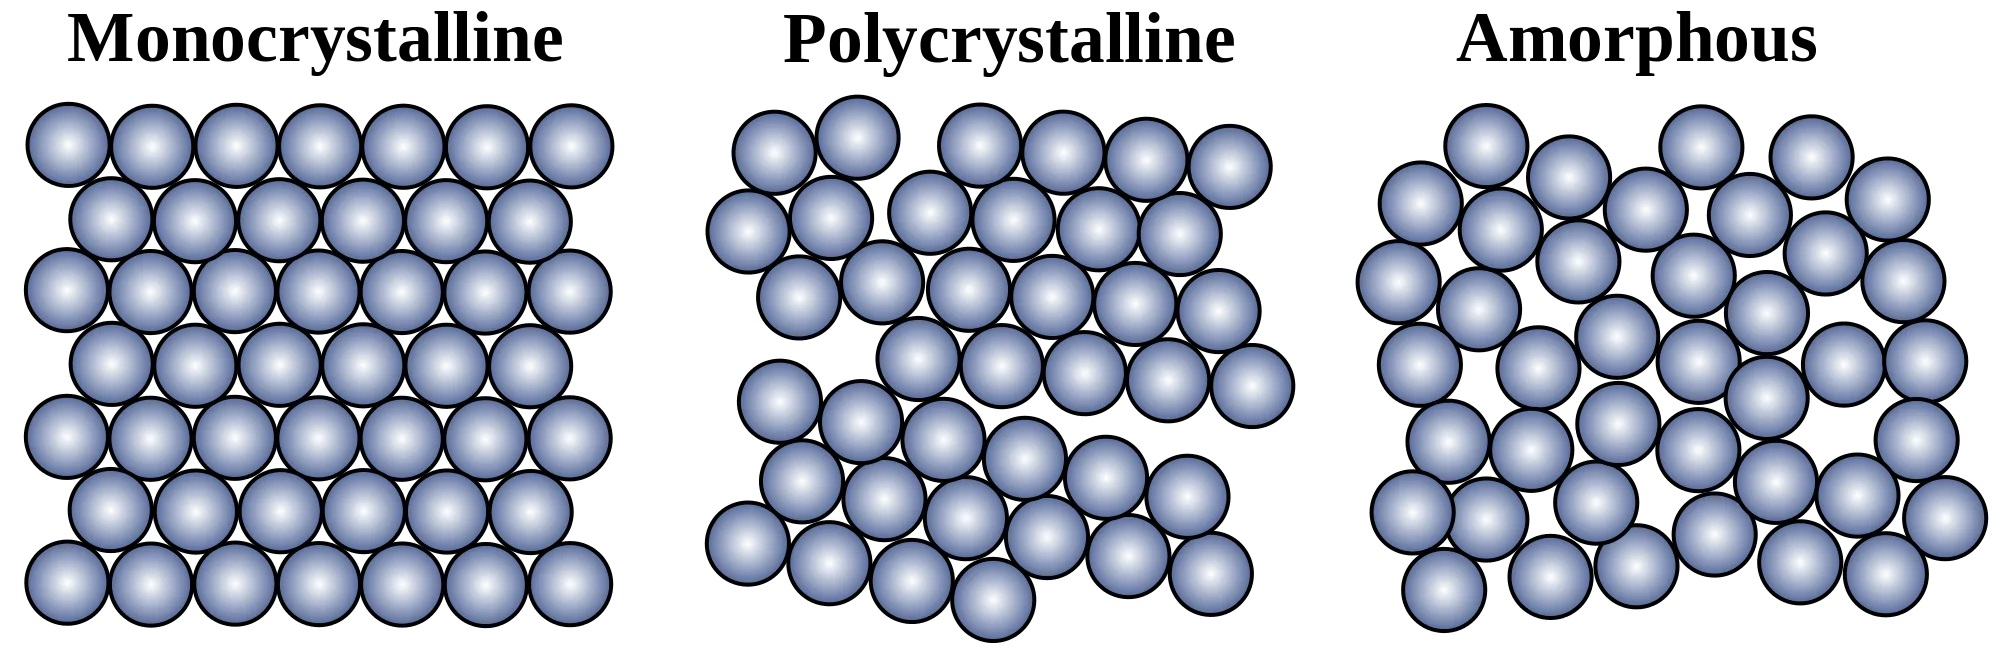
\includegraphics[width=0.8\textwidth]{media/mono_poly_amorph.jpg}
\end{figure*}

\subsection{Directionals dependence of the properties of materials}
\subsubsection{Anisotropy and Isotropy}
\begin{itemize}
  \item Anisotropic: Properties depend on direction (e.g. single crystals, wood, composites)
  \item Isotropic: Properties do not depend on direction (e.g. polycrystalline metals, amorphous materials)
\end{itemize}

\subsubsection{Anisotropy of the Young's Modulus $E$ in most cubic crystals}
In most cases, the $E$ is the largest in the direction of the closest packed atomic planes,
in direction of the space diagonal $\langle 111 \rangle$.

\newpage
\subsubsection{Miller indices for crystal directions}
In short, the Miller indices are the reciprocals of the fractional intercepts
that the plane makes with the crystallographic axes:
\begin{figure*}[ht!]
  \centering
  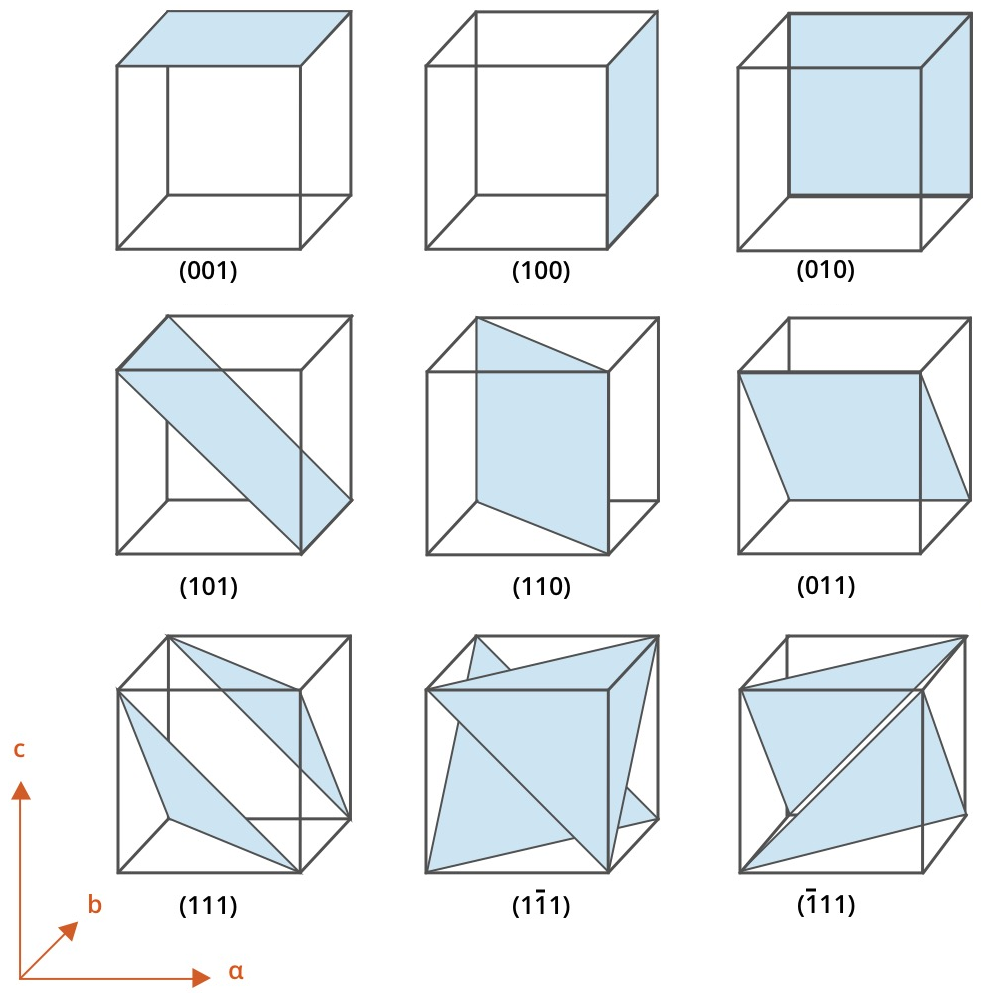
\includegraphics[width=0.5\textwidth]{media/miller_indices.png}
\end{figure*}

\subsection{Directional dependence of properties in polycrystalline materials}
\subsubsection{Polycrystalline materials without texture}
The polycrystalline materials without texture are considered \textbf{quasi-isotropic},
because the grains are randomly oriented.
\begin{figure*}[ht!]
  \centering
  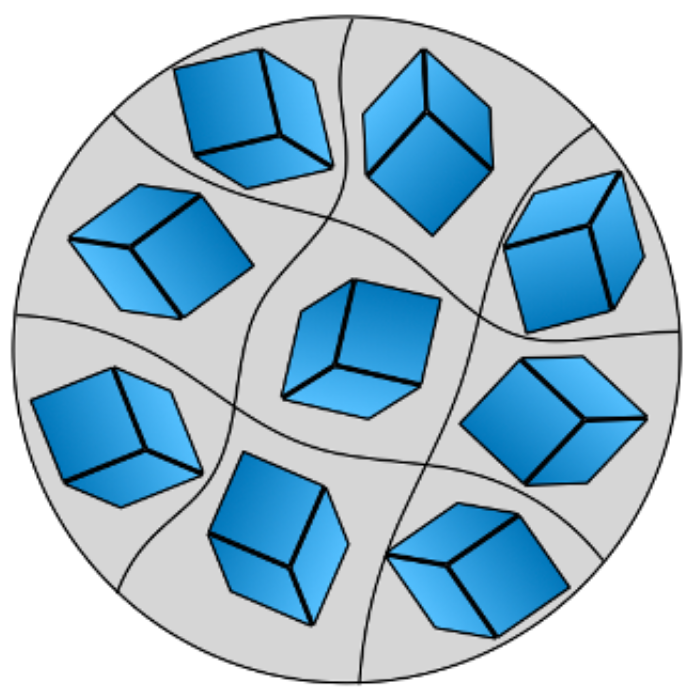
\includegraphics[width=0.1825\textwidth]{media/poly_notexture.png}
  \caption*{Polycrystalline material without texture}
\end{figure*}

\underline{Notice}: each crystal is anisotropic. but the material is quasi-isotropic to the outside, directional
dependence ``averages out''

\subsubsection{Polycrystalline materials with texture}
The polycrystalline materials with texture are considered \textbf{anisotropic},
because the grains are preferentially oriented.
\begin{figure*}[ht!]
  \centering
  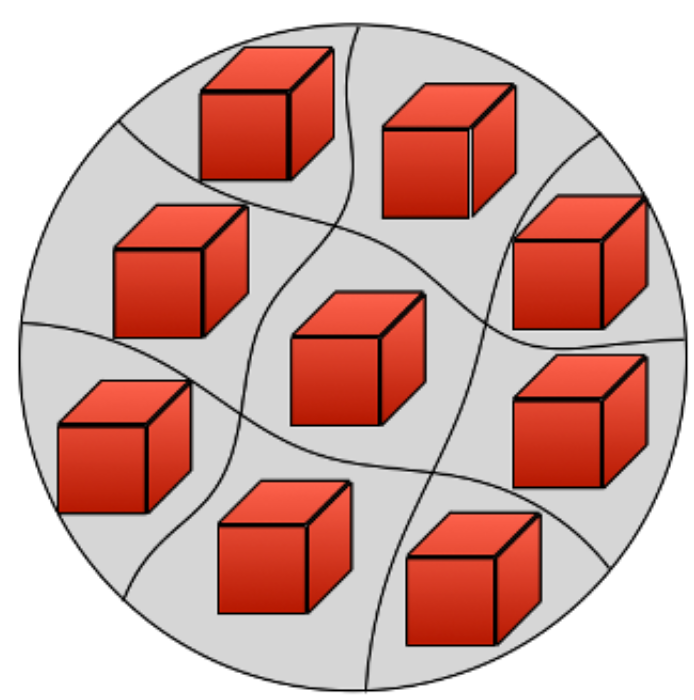
\includegraphics[width=0.1825\textwidth]{media/poly_texture.png}
  \caption*{Polycrystalline material with texture}
\end{figure*}
\newpage

\subsection{Material properties wrap-up}
\subsubsection{Single crystal materials}
\begin{itemize}
  \item \textbf{Anisotropic}
  \item Properties depend on direction
  \item Not uniform = anisotropic
\end{itemize}

\subsubsection{Polycrystalline materials without texture}
\begin{itemize}
  \item \textbf{Quasi-isotropic}
  \item Each crystal: anisotropic
  \item Uniform properties in all directions: isotropic \textrightarrow\ quasi-isotropic
\end{itemize}

\subsubsection{Polycrystalline materials with texture}
\begin{itemize}
  \item \textbf{Anisotropic}
  \item Preferential orientation of the crystallites: texture \textrightarrow\ anisotropic
  \item Examples: rolled and recrystallized electrical sheets with Goss texture
\end{itemize}

\subsubsection{Amorphous materials}
\begin{itemize}
  \item \textbf{Isotropic} (e.g. glass or amorphous metals)
\end{itemize}

\subsection{Polymorphism (Allotropy)}
Some materials may exhibit more than one crystal structure:
\begin{itemize}
  \item Iron $
    \begin{cases}
      \alpha\text{-Fe (ferrite, BCC)} & \text{below } 911^\circ\text{C} \\
      \gamma\text{-Fe (austenite, FCC)} & 911^\circ\text{C} \text{ to } 1392^\circ\text{C} \\
      \delta\text{-Fe (ferrite, BCC)} & 1392^\circ\text{C} \text{ to } 1536^\circ\text{C}
    \end{cases}$
  \item Titanium $
    \begin{cases}
      \text{HCP} & \text{below } 880^\circ\text{C} \\
      \text{BCC} & \text{above } 880^\circ\text{C}
    \end{cases}$
  \item Shape memory alloys (e.g. NiTi)
  \item Carbon (graphite, diamond, graphene, fullerene, CNT, \dots)
  \item Zirconia (high crack resistance due to phase transformation toughening)
  \item Ferro- and piezoelectric materials (e.g. PZT, quartz, \dots)
\end{itemize}

\subsubsection{Polymorphism of Iron (Fe)}
\begin{figure}[ht!]
\centering
\begin{minipage}[t]{0.48\textwidth}
  \centering
  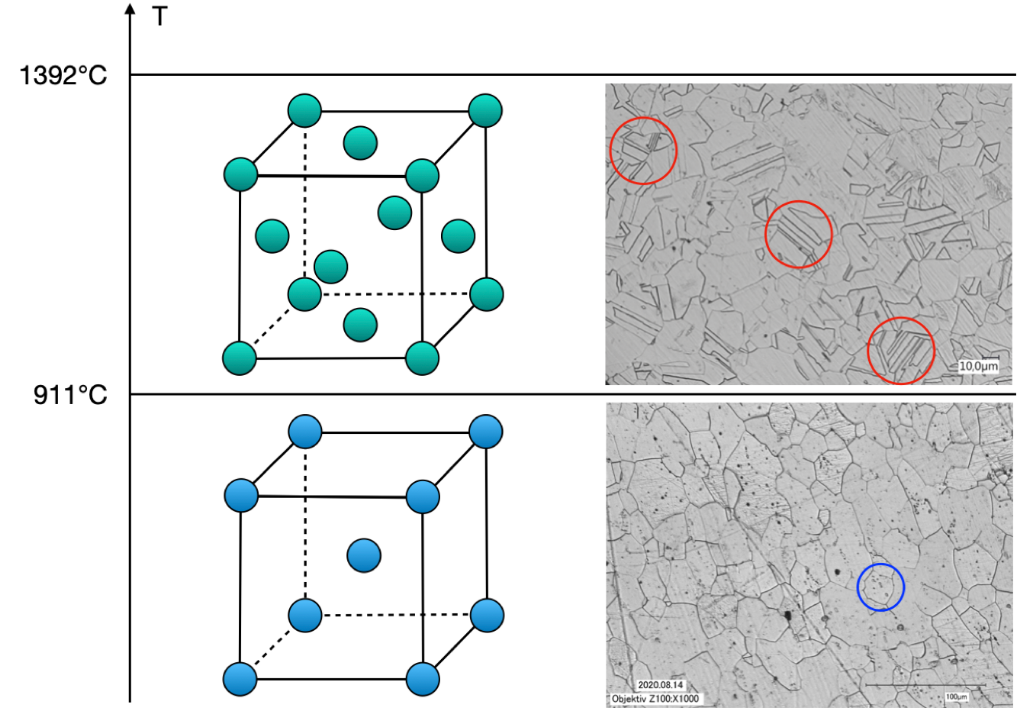
\includegraphics[width=\linewidth]{media/ferrite_trans.png}
  \captionof*{figure}{Slow Austenite transformation in steel: Ferrite}
\end{minipage}\hfill
\begin{minipage}[t]{0.48\textwidth}
  \centering
  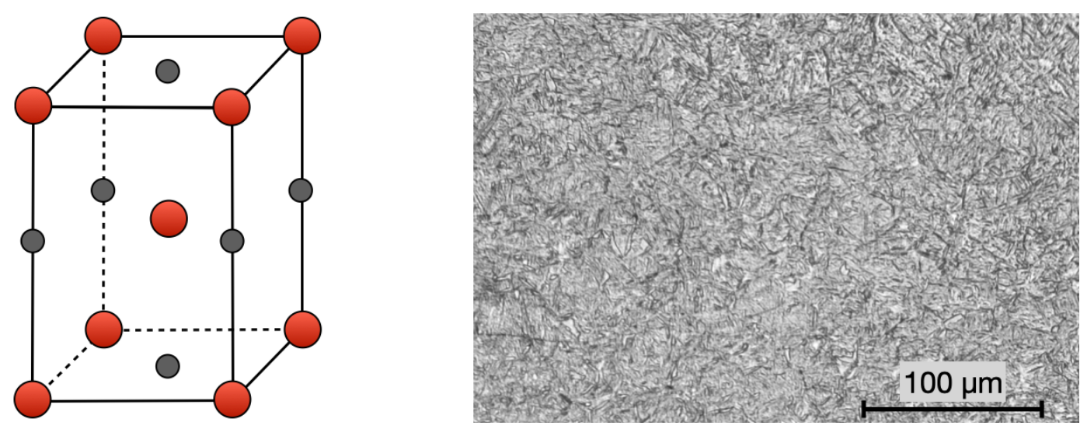
\includegraphics[width=\linewidth]{media/martenesite_trans.png}
  \captionof*{figure}{Fast Austenite transformation: Martensite}
\end{minipage}
\end{figure}

\newpage
\subsubsection{Polymorphism of Carbon (C)}
\forestset{
  mybox/.style={
    draw, rounded corners, align=center, inner sep=4pt, outer sep=2pt
  },
  my edge/.style={-latex}
}

\begin{forest}
for tree={
  mybox,
  edge={-latex},
  l sep=10pt,
  s sep=8pt,
  anchor=north
}
[Carbon
  [Amorphous Carbon
    [Activated Carbon]
    [Templated Carbon]
  ]
  [Crystalline Carbon
    [Graphite
      [Paracrystalline]
      [Rhombic]
      [Hexagonal]
    ]
    [Fullerene]
    [CNT]
    [Carbyne]
    [Diamond
      [Cubic]
      [Hexagonal]
    ]
  ]
]
\end{forest}

\subsubsection{Polymorphism of Nitinol (NiTi)}
NiTi is a shape memory alloy (SMA), used for screen lock of tablet notebooks, medtech,
and spectacle frames.
\begin{figure*}[ht!]
  \centering
  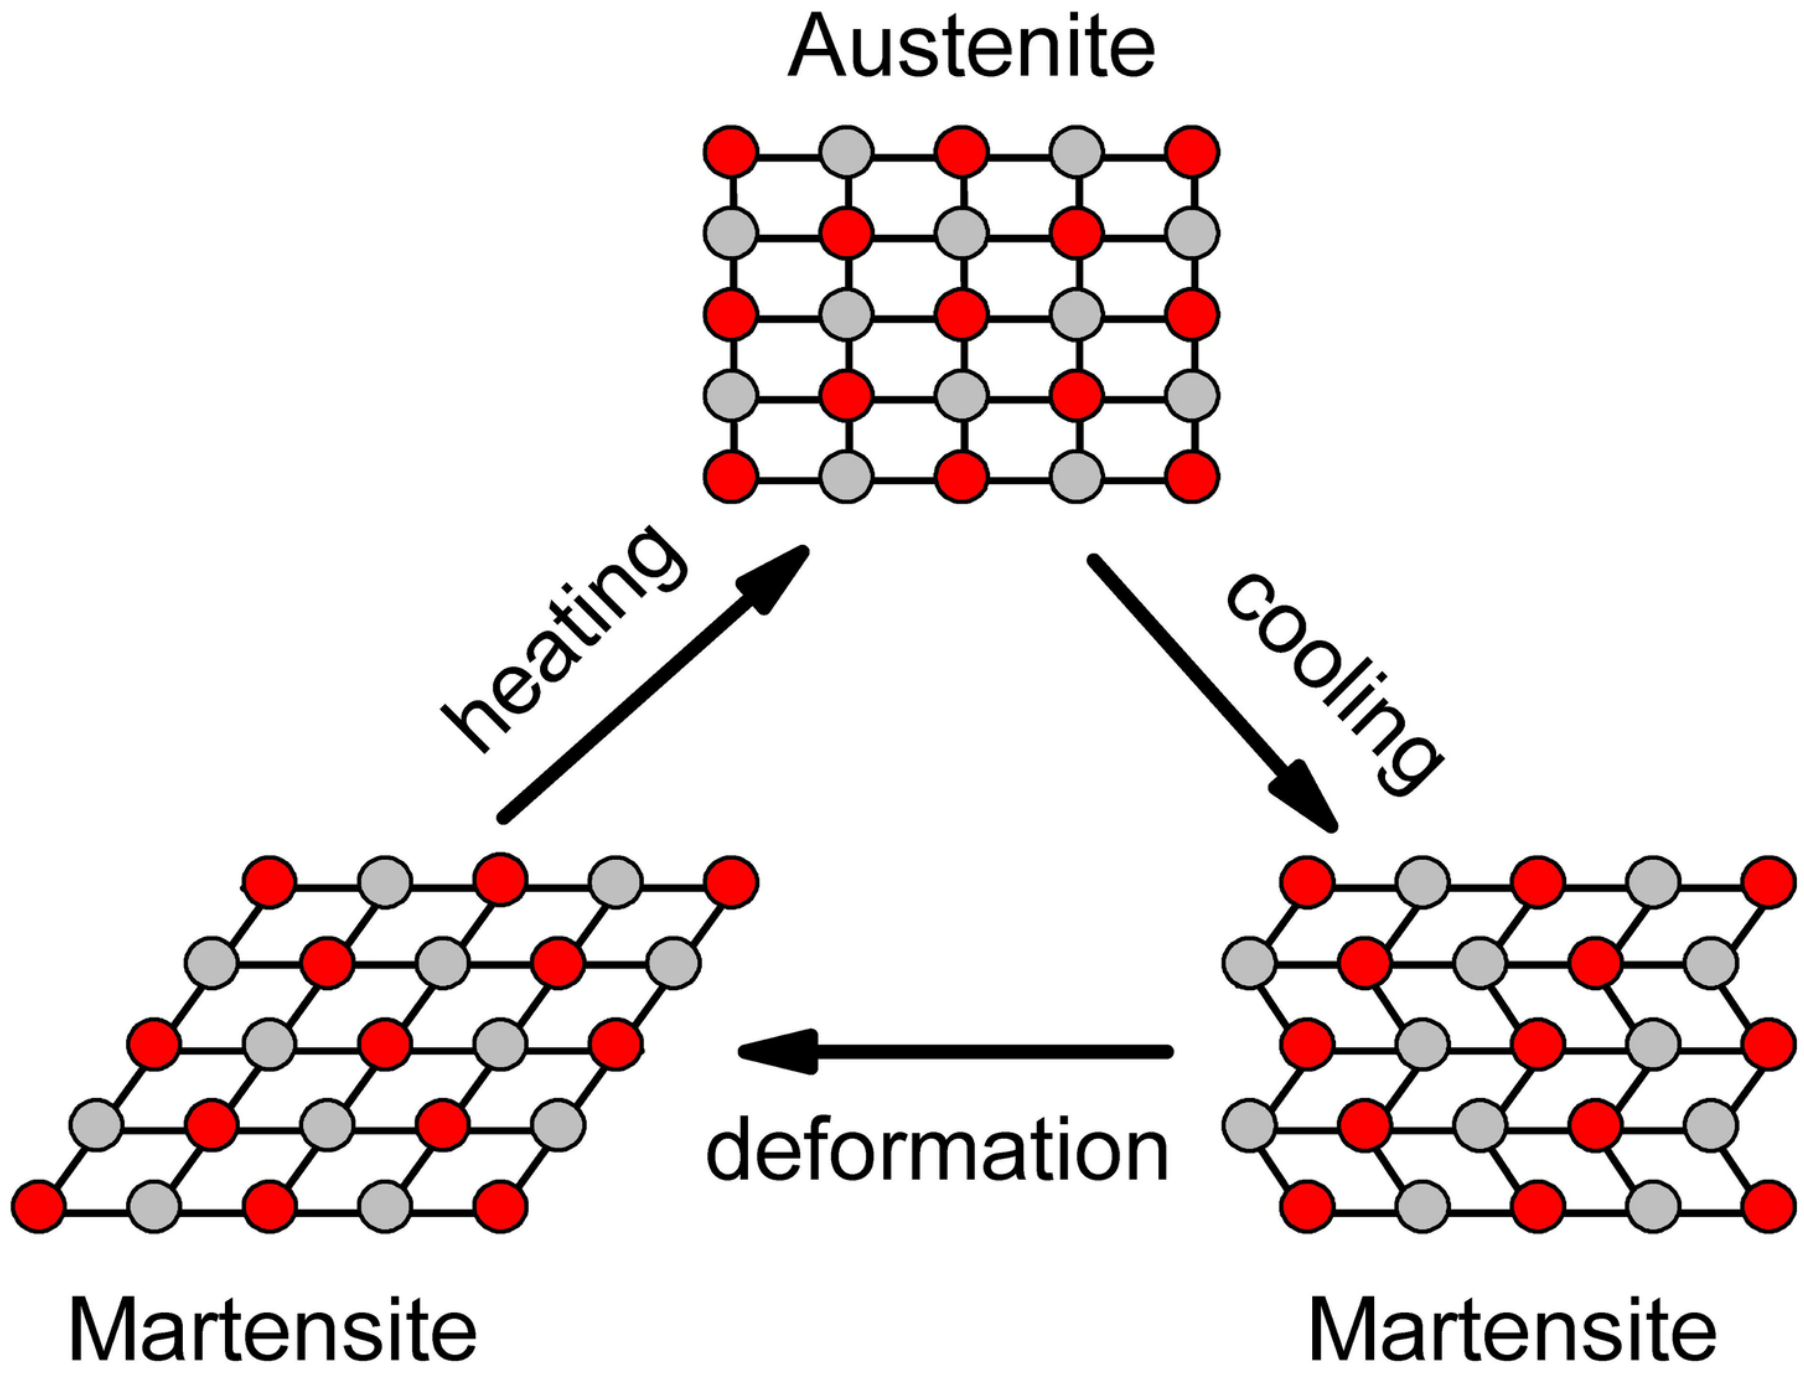
\includegraphics[width=0.4\textwidth]{media/Nitinol.png}
\end{figure*}

\subsection{Microstructure and Phases}
Phases are \textbf{homogeneous} subsections of a material with uniform physical and chemical properties:
\begin{itemize}
  \item A phase can be crystalline or amorphous
  \item At the phase boundaries, a sudden change in structure, properties and chemical composition occurs
\end{itemize}

Polycristalline materials can consist of:
\begin{itemize}
  \item One phase (homogeneous microstructure, e.g. only iron crystals)
  \item Different phases (heterogeneous microstructure, e.g. graphite and iron)
\end{itemize}

\begin{minipage}[t]{0.48\textwidth}
  \subsubsection{Homogeneous microstructure}
  They have only one phase and crystal structure:
  \vspace*{0.8cm}
  \begin{center}
    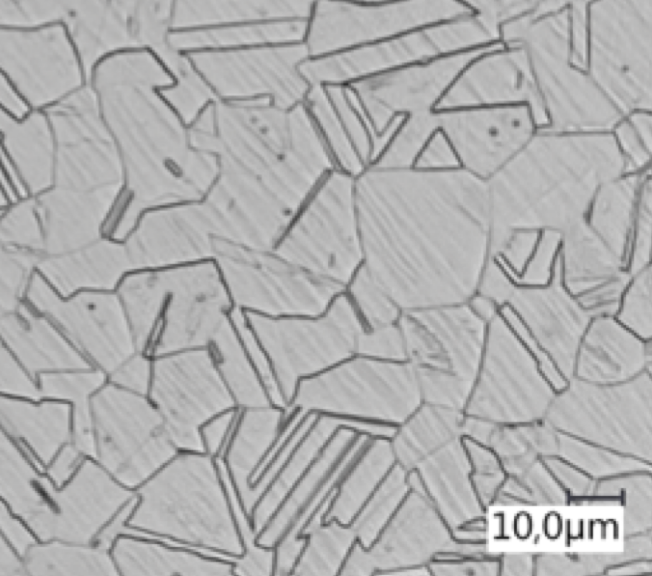
\includegraphics[width=0.65\textwidth]{media/homogeneous_microstructure.png}
  \end{center}
\end{minipage}
\hfill
\begin{minipage}[t]{0.48\textwidth}
  \subsubsection{Heterogeneous microstructure}
  They have multiple phases and many types of crystal structures:
  \vspace*{0.5cm}
  \begin{center}
    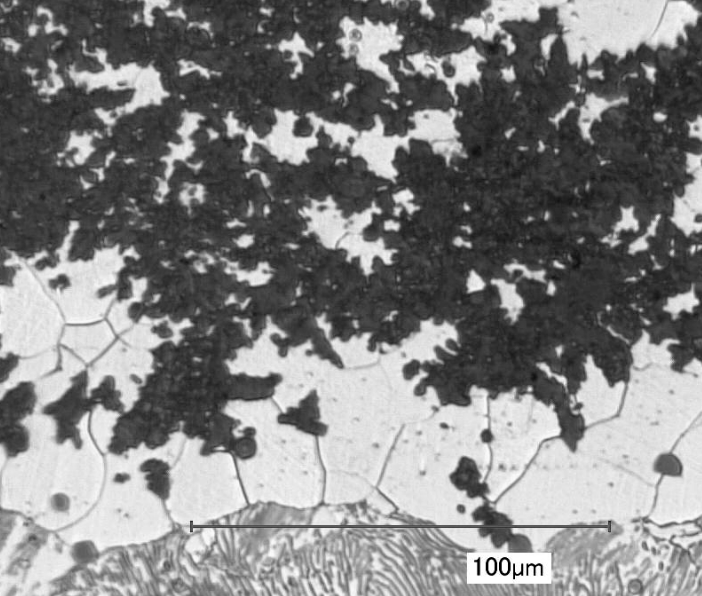
\includegraphics[width=0.7\textwidth]{media/heterogeneous_microstructure.png}
  \end{center}
\end{minipage}

\newpage
\subsection{Alloys}
\subsubsection{Definition of an alloy}
An alloy is a metallic material of at least 2 types of atoms:
\begin{itemize}
  \item Metal + Metal (iron-nickel, gold-silver, tin-lead, aluminum-copper, \dots)
  \item Metal + Non-metal (iron-carbon (steel), nickel-phosphorus, \dots)
\end{itemize}

\subsubsection{Microstructure of alloys}
\begin{itemize}
  \item \textbf{Homogeneous}, single-phase, only one type of cristal: SOLID SOLUTION CRYSTAL
  \item \textbf{Heterogeneous}, multi-phase, MIX OF DIFFERENT CRYSTAL TYPES:
  \begin{itemize}
    \item Crystals of pure metals without impurity atoms (no solid solution crystals)
    \item Solid solution crystals with impurity atoms,
    \item Crystals of intermetallic or intermediate phases (chem compounds crystals with their own distinguished crystal structure e.g. Ni$_3$Ti, Fe$_3$C, \dots)
    \item (Impurity particles, e.g. added ceramic particles or slag residues)
  \end{itemize}
\end{itemize}

\newpage
\section{Most important metal structures and crystal lattice defects}




\newpage
\appendix
\section*{Appendix}
\addcontentsline{toc}{section}{Appendix}

\subsection*{Indices and Abbreviations}
\begin{description}
\item[Amorphous] Non-crystalline material with no long-range order.
\item[Crystalline] Material with atoms arranged in a highly ordered microscopic structure, forming a crystal lattice that extends in all directions.
\item[Monocrystalline] Material consisting of a single crystal or a continuous crystal lattice with no grain boundaries.
\item[Polycrystalline] Material composed of many crystallites of varying size and orientation.
\item[Anisotropy] Direction-dependent properties of a material {\color{red}(Monocrystalline and polycrystalline with texture)}
\item[Isotropy] Direction-independent properties of a material {\color{red}(Amorphous)}
\item[Quasi-isotropy] Approximate isotropy in polycrystalline materials with random grain orientation {\color{red}(Polycrystalline without texture)}
\item[Polymorphism / Allotropy] Ability of a material to exist in more than one form or crystal structure.
\item[Homogeneous] Uniform composition and properties throughout the material.
\item[Heterogeneous] Non-uniform composition and properties throughout the material.
\item[Alloy] A mixture of two or more elements, where at least one element is a metal.
\end{description}

\end{document}
